\section{Apache Storm}
\label{section:storm}

Apache Storm wird vom Hauptentwickler Nathan Marz im Proposal als verteiltes, fehlertolerantes und hochperformantes Echtzeitberechnungssystem definiert. Ursprünglich wurde die Anwendung von der Firma Backtype in 2011 entwickelt. Im gleichen Jahr wurde die Firma Backtype von Twitter übernommen und der Quelltext auf Github \citeint{GitHub} unter dem Repository \textit{storm} \citeint{storm:GitHub} von Nathan Marz veröffentlicht. In 2013 wurde die Aufnahme von Storm in die \gls{glo:asf} geplant. Dazu wurde ein Storm Proposal von Nathan Marz eingereicht. \citeint{storm:apache:stormProposal} 

Seit 2013 befindet sich Storm im Apache Incubation-Prozess \citeint{storm:apache:stormIncubationStatus}. Eine Überführungsversion 0.9.1-incubating wurde dafür eingerichtet. Der Quelltext und das Lizenzmodell wird in die \gls{glo:asf} aufgenommen \citeint{apache:softwareFoundation}. Der Verlauf des Überführungsprozesses zur \gls{glo:asf} wird auf der Incubator-Statusseite \citeint{storm:IncubatorStatusPage} festgehalten. In der Tabelle \ref{tab:vorstorm} wird eine Kurzübersicht über Apache Storm gegeben. Darin wird ein aktiver Entwicklungsstatus angegeben. Die Aktivität wird aus dem GitHub \textit{Contributors-Graph} bei 84 Projektteilnehmern bestimmt \citeint{storm:Contributors}. Zur Entwicklung werden mehrere Sprachen Clojure, Java und Python angegeben. Nathan Marz gibt an Storm in der Programmiersprache Clojure \citeint{clojure} zu entwickeln und mit Java  \citeint{javaAbout} kompatibel zu sein, neben Java und Clojure  findet die Github Sprachen-Suche \citeint{storm:GitHubApacheMirror} im Repository \textit{storm} auch Python \citeint{pythonAbout}. Ab Version 0.9.1-incubating wird eine verbesserte Plattformkompatibilität zum Betriebssystem Microsoft Windows angeboten und die Standardtransportschicht ZeroMq \citeint{zeromq:guide} wurde durch Netty \citeint{netty} ersetzt \citeint{storm:Changelog}.

\begin{table}[htbp]
	\centering
		\begin{tabular}{@{}ll@{}} \toprule
			\textbf{Faktum} & \textbf{Beschreibung} \\ \midrule
			Hauptentwickler & Nathan Marz \\
			Stabile Version & 0.9.1-incubating vom 22.02.2014 \\ 
			Entwicklungsstatus &  Aktiv \\
			Entwicklungsversion & 0.9.2-incubating, 0.9.3-incubating \\
			Sprache & Clojure, Java, Python \\
			Betriebssystem & Platformübergreifend (Microsoft Windows mit Cygwin Umgebung) \\
			Lizenz & Eclipse Public License 1.0 (Incubating Apache License version 2.0) \\
			Webseite &  \citeint{storm:home} \\
			Quelltext & \citeint{storm:GitHubApacheMirror} \\			
			\bottomrule			
		\end{tabular}
	\caption{Kurzübersicht Apache Storm}
	\label{tab:vorstorm}
\end{table}

In Tabelle \ref{tab:bewstorm} werden die Bewertungskriterien aus Kapitel \ref{chapter:analyse} in Apache Storm geprüft. Als Architektur wird die moderne Systemarchitektur Strukturierte Peer-To-Peer-Architektur, die eine horizontale Verteilung unterstützt, angegeben. Apache Storm besteht aus drei Komponenten: \textit{Nimbus}, \textit{Supervisor} und \textit{UI}. Der \textit{Nimbus} stellt die zentrale Stelle und übernimmt die Aufgabe des \textit{Scheduler} - einem Arbeitsplaner. Der \textit{Nimbus} is klein gehalten und verteilt die Aufgaben zwischen den Arbeitsknoten. Die Arbeitsknoten werden in Apache Storm \textit{Supervisor} genannt. Mehrere Supervisor-Instanzen sind in einem Apache Storm Cluster möglich. Die dritte Komponente \textit{UI} visualisiert den momentanen Status der Apache Storm Komponenten \textit{Nimbus} und \textit{Supervisor}. 

Bei der Verarbeitung von Informationen kann in Apache Storm pro Verarbeitungseinheit die Anzahl an benötigten Threads als Argument explizit übergeben werden. Die Konfiguration dazu findet im Quelltext statt. Um eine komplexe Verarbeitung durchzuführen, muss in Apache Storm eine \textit{Topology} implementiert und veröffentlicht werden. Die \textit{Topology} wird auf dem Apache Storm Cluster permanent ausgeführt und kann nicht dynamisch verändert werden. Die Kommunikation erfolgt zwischen den einzelnen Apache Storm Komponenten mit einem zusätzlichen Werkzeug: Apache ZooKeeper \citeint{zookeeper:Home}. Apache ZooKeeper wird als verteilte Synchronisation und Koordination der Aufgaben durch Nimbus auf tieferer Ebene verwendet. Auf der Transportebene kommunizieren Verarbeitungseinheiten durch das asynchrone Client-Server-Framework Netty \citeint{netty}.

Eine komplexe Verarbeitung bzw. Abfrage in einer \textit{Topology} besteht aus \textit{Spouts} und \textit{Bolts}. Die Kommunikation ist dabei einseitig. Ein Empfänger-\textit{Bolt} kann keine Nachricht an einen Sender-\textit{Bolt} zurück schicken. Mit einem \textit{Spout} wird eine externe Datenquelle beschrieben und ein \textit{Spout} liefert eine permanente Folge von ungebunden Tupeln. Ein Tupel ist die Hauptdatenstruktur und kann unterschiedliche Datentypen (integers, longs, shorts, bytes, strings, doubles, floats, booleans und selbstentwickelte) enthalten. Die Folge von ungebundenen Tupeln wird in Apache Storm als \textit{Stream} bezeichnet. Um einen \textit{Spout} zu implementieren reicht es die Schnittstelle \textit{IRichSpout} zu implementieren oder die Klasse \textit{BaseRichSpout} zu erweitern. 

Bei einer Erweiterung von \textit{BaseRichSpout} sind mindestens die Methodenamen \textit{open}, \textit{nextTuple} und \textit{declareOutputFields} zu implementieren. In der Methode \textit{open} kann zum Beispiel eine interne Liste über einen Java-Listener bei einem Dateneingang in einem Datenadapter gefüllt werden. Die Methode \textit{nextTuple} wird jede erste Millisekunde ausgeführt und wenn Nachrichten in der Liste enthalten sind, kann der \textit{SpoutOutputCollector} einen Stream mit einer eindeutigen StreamId und einem Tuple aussenden. Wenn die Nachricht nicht vollständig übertragen wurde, wird über ein \textit{Callback-Methode} \textit{ack} oder \textit{fail} in der implementierten Klasse \textit{Spout} zurückgegeben. Damit wird in Apache Storm sichergestellt, dass die Nachricht mindestens einmal vollständig verarbeitet wurde \citeint{storm:SpoutOutputCollector}. In der Methode \textit{declareOutputFields} wird die Felddefinition der Ausgabe für die weitere Verarbeitung angegeben. \citeint{storm:Spout}

Ein \textit{Bolt} nimmt ein Tupel auf und gibt Tupel wieder aus. Innerhalb eines \textit{Bolt} können Tupel verändert werden. Nachdem Start der \textit{Topology} wird ein \textit{Bolt} erst auf den \textit{Supervisor} übertragen und deserialisiert. \textit{Nimbus} ruft auf der Instanz anschließend die Methode \textit{prepare} auf. In Java muss für die Implementierung eines \textit{Bolt} die Schnittstelle \textit{IBolt} oder \textit{IRichBolt} implementiert werden. Alternativ können auch Basisimplementierungen verwendet werden, wie zum Beispiel \textit{BaseBasicBolt} oder \textit{BaseRichBolt}. Mit der Methode \textit{execute} werden die Tupel angepasst und über den \textit{OutputCollector} ausgesendet. Apache Storm erwartet beim Eingang eines Tupels in einem \textit{Bolt} Bestätigung über die Methode \textit{ack} oder \textit{fail}. Andernfalls kann Apache Storm nicht feststellen, ob eine Nachricht vollständig verarbeitet wurde. \citeint{storm:Bolt}

\begin{figure}[htb!]
\centering
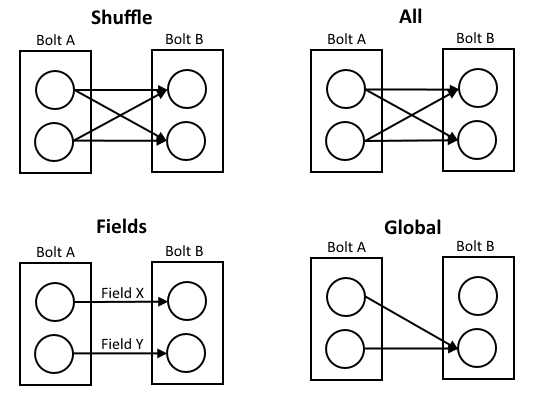
\includegraphics[width=1.0\textwidth]{bilder/stormGroupings.png}
\caption{Apache Storm Gruppierungen
\label{fig:stormGroupings}}
\end{figure}

Durch den \textit{TopologyBuilder} kann eine komplexe Abfrage aus \textit{Spouts} und \textit{Bolts} zusammengesetzt werden. Der \textit{TopologyBuilder} stellt dazu \textit{set}-Methoden für \textit{Spouts} und \textit{Bolts} bereit. Bei dem Setzen eines \textit{Spout} oder eines \textit{Bolt} muss immer eine Referenz-Identifikationsnummer angegeben werden. Durch die Referenz können \textit{Bolt}- oder \textit{Spout}-Komponenten untereinander verbunden werden. Weiterhin kann mit dem Argument \textit{parallelism\_hint} die Anzahl der \textit{Tasks} eingestellt werden, die zur Ausführung benutzt werden. Jeder \textit{Task} wird im Storm Cluster auf einem eigenen \textit{Thread} ausgeführt. Wenn die \textit{setBolt}-Methode aufgerufen wird, wird ein Objekt \textit{InputDeclarer} erzeugt. Darin können verschiedene Gruppierungen (\textit{Shuffle}, \textit{Fields}, \textit{All}, \textit{Global}, \textit{None}, \textit{Direct}, \textit{LocalOrShuffle} \citeint{storm:InputDeclarer}) angegeben werden, um den Stream in definierte Teile zu trennen. In Abbilung \ref{fig:stormGroupings} werden Vier Standardgruppierungen in Apache Storm gezeigt. Mit einem \textit{ShuffleGrouping} werden Tupel eines \textit{Stream} zufällig über die \textit{Tasks} verteilt. Beim \textit{FieldsGrouping} wird der \textit{Stream} durch die Angabe eine Schlagworts getrennt. Tupel mit dem gleichen Schlagwort werden immer an den gleichen \textit{Task} gesendet. Das \textit{AllGrouping} wird auf allen Tasks des \textit{Bolt} repliziert und beim \textit{GlobalGrouping} wird der \textit{Stream} zu einem \textit{Task} gesendet. Weiterhin gibt es noch das \textit{NoneGrouping} bei dem der \textit{Stream} auf dem gleichen \textit{Task} ausgeführt wird und beim \textit{DirectGrouping} entscheidet der \textit{Stream}-Erzeuger auf welchen Konsumenten-\textit{Task} der \textit{Stream} gesendet wird. Durch die Schnittstelle \textit{CustomStreamGrouping} is eine weitere konkrete Implementierung für eine \textit{Grouping}-Strategie möglich. \citeint{storm:TopologyBuilder}

In Apache Storm wird eine Abstraktion \textit{Trident} für eine transaktionsorientierte Abfrage- und Datenverarbeitung bereitgestellt. Mit \textit{Trident} ist es möglich eine Stapelverarbeitung mit Statusinformationen durchzuführen. Es gibt Fünf Ausführungstypen: \textit{Partition-local}, \textit{Repartitioning}, \textit{Aggregation}, \textit{GroupedStreams} und \textit{Merges and Joins}. In \citeint{storm:Trident} wird \textit{Trident} näher erläutert. In den folgenden Absätzen wird kurz auf die möglichen Funktionen mit \textit{Trident} aus \citeint{storm:Trident} eingegangen.

Unter \textit{Partition-local} werden Operatoren (\textit{function}, \textit{filter}, \textit{partitionAggregate}, \textit{partitionPersist}, \textit{projection}) lokal in einem Stapelelement ausgeführt. Die Operatoren \textit{function} und \textit{filter} erben jeweils von der gleichen Basisklasse \textit{BaseFunction}. Bei den Methoden \textit{partitionAggregate} und \textit{partitionPersists} können unterschiedliche Strategien entwickelt werden. Ein neues Aggregat kann mit der \textit{Aggregator}-Schnittstelle oder den erweiterten Schnittstellen \textit{CombinerAggregator} oder \textit{ReducerAggregator} implementiert werden. Um nicht im bestehenden Arbeitsspeicher mit der \textit{MemoryMapState.Factory()} Daten zu speichern, kann über eine konkrete Implementierung der Schnittstelle \textit{IBackingMap} eine neue Strategie zur Datenablage erzeugt werden. Mit \textit{Projection} können Teile der Felder aus einem \textit{Stream} in einem neuen \textit{Stream} unverändert abgebildet werden.

Beim \textit{Repartitioning} kann die Stapelverarbeitung durch \textit{Repartitioning}-Funktionen (\textit{shuffle}, \textit{broadcast}, \textit{partitionBy}, \textit{global}, \textit{batchGlobal}, \textit{partition}) geändert bzw. neu strukturiert werden. Zum Beispiel kann sich die Anzahl der \textit{Tasks} zur parallelen Datenverarbeitung ändern. Mit dem \textit{Repartitioning} ist es möglich die \textit{Tasks} im Cluster neu zu verteilen. Die Methode \textit{groupBy} nutzt \textit{Repartitioning} um den \textit{Stream} mit \textit{partitionBy} neu zu strukturieren. Gruppierte und aggregierte \textit{Streams} können mit bestehenden Apache Storm Primitiven verkettet werden.

\textit{Streams} können in \textit{Trident} durch die spezielle \textit{TridentTopology} zusammengeführt werden. Die \textit{TridentTopology} bietet dazu die Methoden \textit{merge} und \textit{join} an. Beide Methoden erzeugen jeweils einen neu kombinierten \textit{Stream}. Eine Zusammenführung in einem Zeitfenster, dem \textit{Windows Join}, kann mit Hilfe von \textit{partitionPersist} und \textit{stateQuery} durchgeführt werden. Mit \textit{partitionPersist} wird ein \textit{Stream} nach der Identität, die im \textit{join} referenziert wird, zerlegt und in einem Statusstapel mit der Methode \textit{makeState} in der \textit{TridentTopology} ein Status erzeugt werden. Der neue \textit{Stream} steht dadurch permanent für eine Stapelverarbeitung über das \textit{stateQuery} durch \textit{lookup}-Abfragen auf die Identität bereit. 

In der Archivdatei des Quelltextes von Apache Storm \citeint{storm:GitHubApacheMirror} ist im Unterverzeichnis \textit{Example} eine Beispielanwendung \textit{\textit{WordCountTopology.java}} vollständig hinterlegt. Im Anhang \ref{section:quelltext} wird dazu ein Beispiel-Quelltext \ref{lst:WordCountTopology} zum Wortzählen ausgegeben. Der Quelltext stellt einen Auszug des Java-Projekts \textit{storm-starter} aus dem gleichen Verzeichnis dar. In der Methode \textit{main} wird die \textit{Topology} mit einem \textit{RandomSentenceSpout} und Zwei \textit{Bolts}, einem \textit{SplitSentence} und einem \textit{WordCount} erzeugt. Der \textit{RandomSentenceSpout} bekommt Fünf \textit{Tasks} zugeordnet und erhält die Identität "`spout"'. Der \textit{Bolt} \textit{SplitSentence} ist eine \textit{ShellBolt} in dem das Teilen der Satzes in einzelne Worte in der externen Programmiersprache Python über die Kommandozeile angestoßen wird. Beim ersten \textit{Bolt} wird \textit{SplitSentence} auf den \textit{Stream} "`spout"' mit Acht \textit{Tasks}, einem \textit{ShuffleGrouping} und der Identität "`split"' angewendet. Der zweite \textit{Bolt} nimmt den \textit{Stream} "`spout"' aus dem ersten \textit{Bolt} auf und zählt die Worte im \textit{Bolt} \textit{WordCount}, mit Zwölf \textit{Tasks}, einem \textit{FieldGrouping} und der Identität "`count"'. Das \textit{FieldGrouping} von \textit{WordCount} wird nach dem Feld "`word"' gruppiert und der Ausgabestrom enthält nach einer Verarbeitung die Anzahl eines Wortes als Schlüssel-Wert-Paar. Abschließend prüft eine Bedingung, ob die \textit{Topology} im \textit{local cluster mode} zum Debuggen, dem Fehlerlösen durch Haltepunkte, auf dem lokalen Rechner oder in einem Storm Cluster ausgeführt werden soll.

Eine \textit{Topology} hat spezielle \textit{acker}-\textit{Tasks} die die Verarbeitung der \textit{Bolts} und \textit{Spouts} überwachen. Wenn ein Abfragegraph vollständig abgearbeitet wurde, dann wird an das auslösende \textit{Spout} vom \textit{acker}-\textit{Task} die Nachricht gesendet. In dem \textit{Spout} wird die \textit{Callback}-Methode \textit{ack} oder \textit{fail} anschließend verarbeitet. Zusätzlich wird in der \textit{Storm UI} die Anzahl der Nachrichten zu \textit{ack} und \textit{fail} in der Summe dargestellt. Bei Ausfall eines Tasks bekommt der Wurzelknoten eines Abfragegraphens einen "`timeout"' und der Abfragegraph wird "`replayed"', also erneut abgearbeitet. Bei Absturz eines Spout Tasks muss das Warteschlangensystem dafür sorgen, sobald der Spout Task wieder verfügbar ist, die Nachrichten in der Quelle bereitzustellen. \citeint{storm:FullyProcessed}

\begin{table}[ht!]
	\centering
		\begin{tabular}{@{}ll@{}} \toprule
			\textbf{Kriterium} & \textbf{Bewertung} \\ \midrule
			Architektur & Strukturierte Peer-to-Peer-Architektur \\
			Prozesse und Threads & Client-Server Cluster \\
			Kommunikation & TCP-basiert mit Apache Zookeeper \\
			Namenssystem & Hierarchische Benennung \\
			Synchronisierung & Zentralisierter Algorithmus \\
			Pipelining und Materialisierung & Methodenverkettung \\
			Konsistenz und Replikation & Reliability Algorithmus \\
			Fehlertoleranz & Fail-Fast Strategie unter Supervision \\
			Sicherheit & Nur eigene Maßnahmen \\
			Erweiterung & Eigenentwicklung und Community-Beiträge \\
			Qualität & Guaranteeing message processing \\
			\bottomrule			
		\end{tabular}
	\caption{Bewertung Apache Storm}
	\label{tab:bewstorm}
\end{table}

In Apache Storm können der \textit{Worker}, die \textit{Node}, der \textit{Nimbus}- oder \textit{Supervisor}-Dienst abstürzen. Der \textit{Worker} wird vom \textit{Supervisor} neugestartet falls der \textit{Worker} einen Fehler hat. Der \textit{Nimbus} leitet die Abfrage an eine andere Maschine, wenn der \textit{Supervisor} den \textit{Worker} nicht neugestartet bekommt. Sobald eine Node ausfällt, startet \textit{Nimbus} die \textit{Tasks} auf einer anderen Maschine. Da beide Dienste in einem Fehlerfall schnell ausfallen und keinen Statusmonitor für einen Ausfall anbieten, ist ein externes \textit{Monitoring} (nagios \citeint{nagios:Monitoring}) und ein \textit{Superversion} (supervisord \citeint{supervisor:ProcessControlSystem}) der Anwendungsdienste \textit{Nimbus} und \textit{Supervisor} notwendig. Nachdem der \textit{Nimbus}- oder \textit{Supervisor}-Prozess durch den Supervisiondienst neugestartet wurde, können neue \textit{Tasks} zu den laufenden \textit{Tasks} auf den \textit{Workern} hinzugefügt werden. \citeint{storm:FaultTolerance}

Die Sicherheit unter Apache Storm wird bisher nur durch Einsatz zusätzlicher Administration des Anwendungssystems erreicht. Auf der Netzwerkebene müssen \gls{glo:ip}-Verbindungen mit \gls{glo:ipsec} gesichert werden. Eine Authentifizierung zwischen den Apache Storm Komponenten und zwischen Apache Zookeeper ist nicht vorhanden. Daher können auf der Anwendungsebene spezifische Richtlinien durch \glspl{glo:acl} umgesetzt werden. \citeint{storm:Security}

Da der Quelltext der Hauptanwendung öffentlich ist, können spezifische Implementierungen in einem separaten Repository hinzugefügt werden. Apache Storm gibt eine Garantie auf Nachrichtenverarbeitung, wie in \citeint{storm:FullyProcessed} gezeigt. Ein \gls{glo:qos} kann durch die Unterstützung des \textit{Monitoring} iterativ entwickelt werden. Ein komplexes \gls{glo:qos}-System ist in Apache Storm nicht vorhanden.

Apache Storm wurde zu Beginn kurz vorgestellt und anschließend durch die Bewertungskriterien genauer erläutert. Es wurden spezifische Begriffe in Apache Storm vorgestellt und in einer Anwendung WordCount gezeigt. Das Erstellen einer Anwendung ist in wenigen Klassen erledigt. Das Debuggen lässt sich in einem lokalen Clustermodus erledigen. Das Veröffentlichen eine Anwendung ist in einem Kommandozeilenaufruf ausgeführt. Die Sicherheit und \gls{glo:qos} sind weniger bis nicht vorhanden. Trotzdem lässt sich ein Cluster mit wenig Konfigurationsaufwand aufbauen und vertikal durch Apache Zookeeper skalieren. Im folgenden Kapitel wird Apache Kafka eingeführt.

%Monitor NASDAQ stocks between $20 and $200 that have moved down more than 2% in the last 20 minutes